\section{Introduction}

With the advent of Internet of Things, the evolution of mobile computing, and the emergence of real-time applications, the processing of an exponentially increasing volume of data must be performed in a timely fashion, i.e., with minimum latency. Despite the elasticity and vast computing power of existing cloud platforms, the access to these resources involves multiple hops of network communication, adding to the latency in which requisitions are processed. Such limitation has the following implications:

\begin{enumerate}

\item Today's deployment of backend services to the cloud may fail to satisfy the requirements of real-time and delay-sensitive client applications; and

\item Offloading of delay-sensitive computation from devices with constrained resources to cloud servers is unlikely to work

\end{enumerate}

To reduce network latency, data processing must be performed closer to where it is produced and consumed. In accordance with this principle, the emerging paradigm of edge computing~\cite{} states that computing power should be pushed from centralized datacenters to the edge of the network. The realization of edge computing, however, still poses many challenges. 

Firstly, the highly distributed edge infrastructure is not expected to exhibit virtually unlimited resources as cloud infrastructure. This limitation requires an efficient use of edge resources and existing models and technologies adopted by cloud providers may not be feasible with edge computing.

Secondly, in contrast with fixed cloud endpoints, mobile applications must rely on a runtime mechanism to discover and negotiate the use of nearby edge servers following an opportunistic and automated approach. Also, as different servers may exhibit different loads, the decision of which edge servers to use must consider their current usage and the application requirements.

Thirdly, cloud servers should not be disregarded. Firstly, because client applications may still rely on cloud backends for non delay-sensitive features. Additionally, edge servers may not be available in the area where the client is located. 

Finally, to avoid increasing the burden of application development, application features to be pushed to the network edge should follow, to the extent possible, a common architecture and implementation.  

\subsection{Motivation}

\subsubsection{Realtime Applications}

The main motivation for displacing computation from cloud to edge servers is to avoid network latency. In specific, real-time applications are the main candidates for benefiting of services deployed at proximal edge infrastructure.

For example, augmented reality (AR) is a type of application that enrich users view of the physical world with virtual elements like information about buildings and monuments or tips to help users to achieve physical tasks. AR applications commonly depend on two key computational tasks: 1) extracting features from physical elements in the captured scene; and 2) matching these features against a feature database to obtain the corresponding information. 

With the advent of mobile computing,  mobile augmented reality (MAR) applications can be deployed to companion devices like smartphones and tablets. Nonetheless, MAR applications relying on data that is too large or too frequently updated to be ported to devices must rely on external servers. As MAR applications captures live representation of the physical world, this reality must be augmented at runtime, meaning data must be retrieved in a timely fashion. Due to network latency, a cloud-based solution tends to fail. Accordingly, feature extraction task should be deployed near to client devices, e.g.., to edge servers. 

\begin{figure}[htbp]
\centering
\subfloat[first caption.\label{fig:cloud-to-edge}]{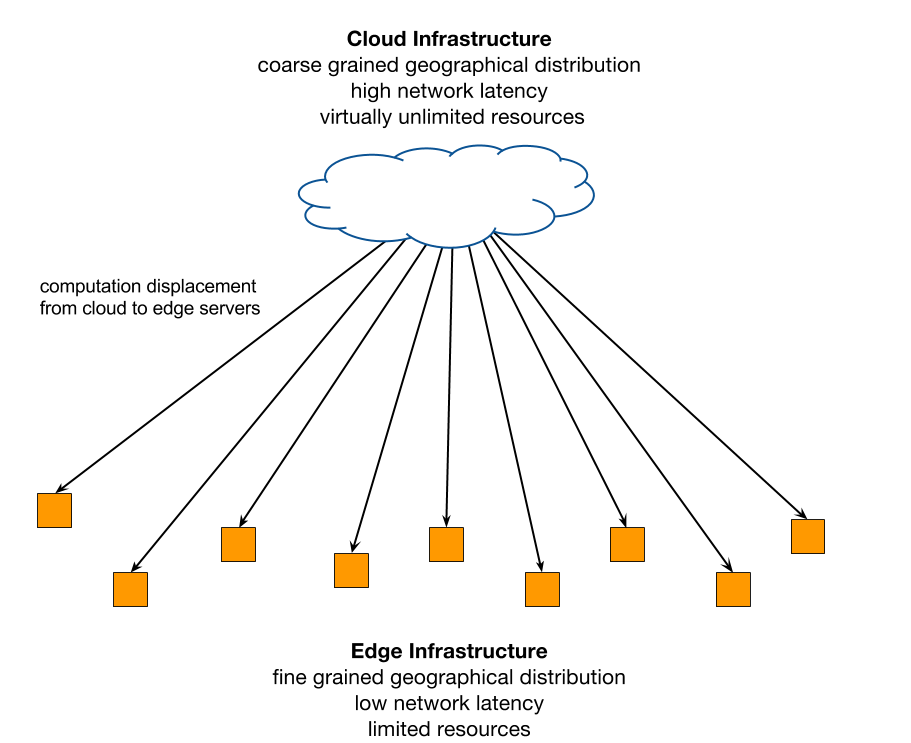
\includegraphics[width=0.49\textwidth]{figs/cloud-to-edge.png}}\hfill
\subfloat[second caption.\label{fig:mobile-to-edge}] {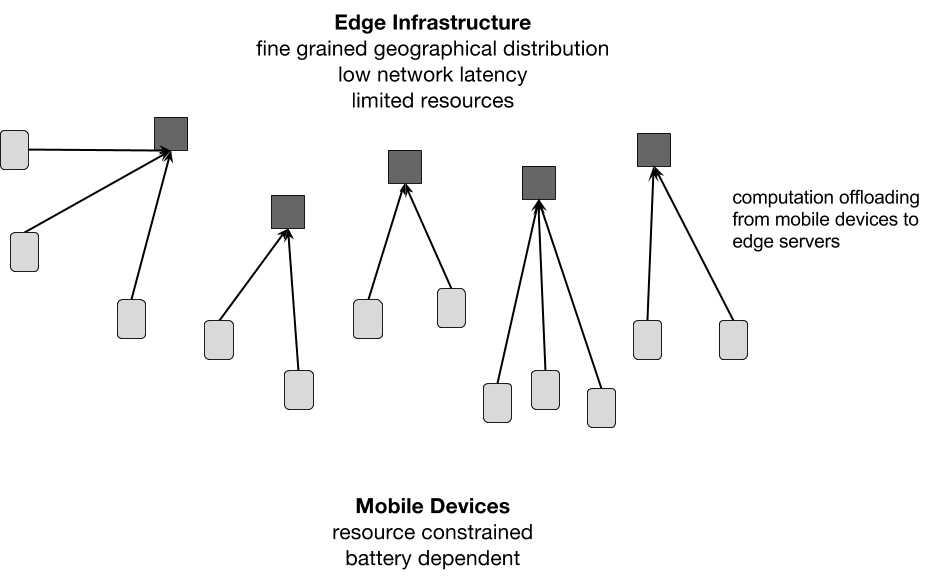
\includegraphics[width=0.49\textwidth]{figs/mobile-to-edge.png}}\hfill

\caption{General caption.} \label{fig:1}
\end{figure}


\subsubsection{Mobile Computation Offloading}

In addition to the problem of network latency, mobile devices exhibit limitations that may further motivate the use of edge computing. 

For instance, some mobile applications rely on heavyweight tasks that can overstress the platform and limit the concurrent execution of other applications. Moreover, battery is a valuable resource that may be significantly affected by the kind of computation performed by mobile devices. 

In previous works~\cite{Mobile Cloud Computing}, this problem had been addressed with the offloading of mobile computation to cloud servers. This solution, however, is limited by network latency.

The paradigm of edge computing can be explored to mitigate the problems related to the resource limitations of mobile devices. For this, heavyweight computation from mobile applications could be offloaded to nearby edge servers. 

As an example, the previously mentioned feature extraction task from MAR applications is an example of a heavyweight computation based on image processing. Instead of performing it locally, mobile devices could offload it to nearby edge servers. 

\subsection{Serverless Computing}

Serverless computing emerged as a new execution model for cloud computing in which server management and capacity planning decisions are hidden from the software application engineers. In this model, serverless providers dynamically manage the allocation of machine resources. Multiple vendors are now offering serverless compute runtime and database services. 

Among its main advantages, the serverless model is considered to be cost-efficient in comparison to virtual machine and container-based provisioning models, which generally involve significant periods of underutilization or idle time. As it has been argued elsewhere~\cite{ESOCC'17}, a serverless architecture can be employed to enable low-latency applications to make use of edge computing computational resources in an efficient and scalable way. Additionally, mobile devices could make use of compute runtimes deployed at nearby edge servers to extend their capabilities. Notwithstanding the potential of such combination, a complete model for its realization is still missing. 

\subsection{Contribution}

In this work, we propose a unified model for the the provisioning of different kinds of edge infrastructure as a service. We also specify a reference architecture based on the paradigm of serverless computing. The proposed architecture is suitable for both cloud and edge infrastructures, reducing the burden of application development. Finally, we evaluated our model and architecture with two scenarios of edge computing: one in which edge servers are located at cellular infrastructure, and another in which edge servers are located indoors at an office building. The results showed the feasibility and scalability of providing edge infrastructure as a service.

TODOs: 
\begin{itemize}

\item add a critical application class example
\item introduce the concept of edge continuum

\end{itemize}

This paper is organized as follows...




